% v2-acmlarge-sample.tex, dated March 6 2012
% This is a sample file for ACM large trim journals
%
% Compilation using 'acmlarge.cls' - version 1.3, Aptara Inc.
% (c) 2011 Association for Computing Machinery (ACM)
%
% Questions/Suggestions/Feedback should be addressed to => "acmtexsupport@aptaracorp.com".
% Users can also go through the FAQs available on the journal's submission webpage.
%
% Steps to compile: latex, bibtex, latex latex
%
%%\documentclass{acmtog} % V1.2
\documentclass[prodmode,acmjetc]{acmsmall}
%%\documentclass[prodmode,acmtecs]{acmsmall}

%\acmVolume{VV}
%\acmNumber{N}
%\acmYear{YYYY}
%\acmMonth{Month}
%\acmArticleNum{XXX}
%\acmdoi{10.1145/XXXXXXX.YYYYYYY}

\acmVolume{99}
\acmNumber{9}
\acmYear{2018}
\acmMonth{9}
\acmArticle{999}%%for use with the acmsmall document class

%\acmVolume{99}
%\acmNumber{9}
%\acmYear{2018}
%\acmMonth{September 25}
%\acmArticle{999}%%for use with the acmsmall document class
%\acmArticleNum{999}%%For use with the acmtog document class
%\acmdoi{10.1145/0000000.0000000}%%For use with the acmtog document class

\usepackage{bm, amsmath, float}
\usepackage{verbatim}
\usepackage{hyperref}
\usepackage{csquotes}


\hypersetup{
    colorlinks=true,
    linkcolor=blue,
    filecolor=magenta,      
    urlcolor=cyan,
    citecolor = blue
}

\usepackage[ruled]{algorithm2e}
\renewcommand{\algorithmcfname}{ALGORITHM}
\SetAlFnt{\small}
\SetAlCapFnt{\small}
\SetAlCapNameFnt{\small}
\SetAlCapHSkip{0pt}
\IncMargin{-\parindent}

\renewcommand{\labelitemi}{$\bullet$}


\begin{document}

\markboth{R. D. Reese}{Issues in Level-of-Detail Based Rendering Using Compute Shaders and Data Buffers}

\title{Issues in Level-of-Detail Based Rendering Using Compute Shaders and Data Buffers} % title

\author{RANDALL D. REESE %%{\upshape and} MANUEL M. OLIVEIRA
\affil{Idaho National Laboratory}
%\and
%GLADIMIR V. G. BARANOSKI
%\affil{University of Waterloo}
%\and
%SEAN FOGARTY
%\affil{University of Illinois at Urbana-Champaign}
% NOTE! Affiliations placed here should be for the institution where the
%       BULK of the research was done. If the author has gone to a new
%       institution, before publication, the (above) affiliation should NOT be changed.
%       The authors 'current' address may be given in the "Author's addresses:" block (below).
%       So for example, Mr. Fogarty, the bulk of the research was done at UIUC, and he is
%       currently affiliated with NASA.
}

\category{I.3.7}{Computer Graphics}{Three-Dimensional Graphics and Realism}[Animation]
\category{I.3.5}{Computer Graphics}{Computational Geometry and Object Modeling}[Physically based modeling]

\terms{Volumetric rendering, Exascale visualization}

\keywords{Level of detail, Unity, Compute shader}

\acmformat{Randall D. Reese. 2018. Issues in Level-of-Detail Based Rendering Using Compute Shaders
{\em ACM Trans. Graph.} 99, 9, Article 999 (September 2018), 999 pages.\\
\doiline}



\begin{abstract}
Rendering large scale volumetric data sets via compute shaders requires substantial buffer space. We discuss issues arising from determining a proper level of detail (LOD) for each 
volumetric brick when rendered using a compute shader in commodity game engine software. It is argued that numerous difficulties arise from attempting to render volumes with a 
render-time-dependent LOD. One significant concern is the loss of acceptable frames-per-second rendering rates. The long-term feasibility of rendering volumes using a compute 
shader is brought into question. 
\end{abstract}

\begin{bottomstuff}
%%This work is supported by the Widget Corporation Grant \#312-001.\\
Author's address: Randall Reese, 995 University Blvd. MS 3553, Idaho Falls, ID 83401; email: randall.reese@inl.gov.
\end{bottomstuff}




% At a minimum you need to supply the author names, year and a title.
% IMPORTANT:
% Full first names whenever they are known, surname last, followed by a period.
% In the case of two authors, 'and' is placed between them.
% In the case of three or more authors, the serial comma is used, that is, all author names
% except the last one but including the penultimate author's name are followed by a comma,
% and then 'and' is placed before the final author's name.
% If only first and middle initials are known, then each initial
% is followed by a period and they are separated by a space.
% The remaining information (journal title, volume, article number, date, etc.) is 'auto-generated'.

\maketitle



% Head 1
\section{Introduction}

Herein we examine some thoughts on an extension of the volumetric rendering techniques presented in \cite{PEARC18} and \cite{Sterbentz2018}. This work is born out of the author's various attempts to overcome issues of extreme data size, memory restraints, and data streaming. 
Throughout the remainder of this work, we will assume that all data sets spoken of have been previously curved into a hierarchical Z-curve, on a per-brick basis. At times, we will 
refer to ``raw data" or ``raw brick data" being loaded into buffers. 
These uses of the word ``raw" are in reference to the actual \texttt{<brickNumber>.hz} files being loaded into buffers, not the lack of an HZ-leveling being enforced on the data. 
Each brick is loaded from an individual \texttt{.hz} file that contains the data for each voxel comprising the given brick. A single JSON meta-file associated with the volume as a 
whole provides further rendering information for each individual brick.
It will also be assumed that readers are familiar with concepts of 
bricking, ray-tracing, HZ-curve ordering, and basic Unity development.  

In order to use the compute shader to render a volume, we must load the raw brick data into 
\texttt{RWStructuredBuffer}s of unsigned integers (\texttt{unit}). Currently the entirety of the brick data is loaded fully into the buffers. This means that the potential for 
buffer overflow exists when the volume being rendered is large (e.g. the Gray Rot data discussed in \cite{Sterbentz2018}). On smaller data sets, the hazard of buffer overflow is not of concern. 






We now discuss several issues with loading larger data sets for rendering via compute shaders. 
Section \ref{scale} explains how we overcame an issue of scaling the volumes upon initial rendering. 
In Section \ref{LODcull}, we consider several attempts to solve the aforementioned issues of buffer overflow.  
This is followed by our outlaying in Section \ref{shells} a method using so called ``shells" of bricks. Section \ref{SIEVAS} briefly outlines some of the aspects of 
using the SIEVAS data management system (see \cite{SIEVAS}) to stream brick data. These first five sections are the result of a notes taking process by the author 
and are meant not as final declarations of outcomes, but rather should be seen as documentation of an ongoing process of attempting to expand upon the volume 
visualizer tool introduced in \cite{PEARC18} and \cite{Sterbentz2018}.  The final section (Section \ref{issues}) of this paper is devoted to several discussions on 
a variety of issues in volume visualization. 
These discussions are written as summaries of the issues discovered in developing the work presented in Sections \ref{scale} through \ref{SIEVAS}. An understanding 
of each of these issues is critical if one wishes to pursue further work on  volume visualization. 
Section \ref{conclude} provides a short synopsis of the current state of the volume visualizer. 


 

\section{Inherent scale in raw HZ-leveled data}\label{scale}
In Unity, each brick is represented by a cube \texttt{GameObject}. 
However, unlike the fragment shader (which uses no buffers), the compute shader employs \texttt{RWStructuredBuffer}s of \texttt{uint}s to hold the raw brick data for rendering. 
While we previously were able to scale (using the \texttt{GameObject.Transform.localscale} property) the cube \texttt{GameObject} to the appropriate scale (as determined by the 
volume specific meta-file), because the compute shader must read raw voxel data from a buffer when performing the final render, all previously enforced scaling is lost. We refer to 
this as the ``inherent" scale of the data.  When the desired scale of the volume is not 1:1:1  (X:Y:Z), the inherent scale of the data will not match the desired scale of the 
volume. In order to ameliorate this discrepancy, we must apply a transfer mapping to the individual rays employed in the ray-tracing algorithm. This is accomplished by representing  
the current position on a given ray as a vector in 3-space, then applying a simple linear transformation, $T$, to the vector in question. If $\bm{r} = (x_0, y_0, z_0)$ is the 
current position of the ray in 3-space, this can be written as follows:
\[T(\bm{r}) = S^{-1}\bm{r},\]
where $S$ is a $3 \times 3$ diagonal matrix with the $x$-, $y$-, and $z$-scaling factors on its diagonal. The raw buffer data is then sampled for the voxel nearest to the position 
associated with $T(\bm{r})$. In order to better fit the volume to the viewing window, it is also recommended that the scale vector first be itself scaled to have its smallest entry 
equal to one. (Simply dividing each entry of the scale vector by the minimum component will accomplish this).
 

\section{Attempts at overcoming buffer overflow with culling}\label{LODcull}
As previously discussed, when the brick data is small, the entirety of the volume can be loaded into buffers. However, when the data is 10s or even 100s of gigabytes large, loading 
the whole data set into buffers will likely prove challenging or impossible on most platforms. 
(This is obviously largely dependent on your hardware. Loading 10 or 15 GB into buffers on a high performance machine is likely reasonably achievable). 
One proposed method for overcoming this challenge is loading each brick at a lower level of detail 
(LOD) than that given by the highest Z-level in the HZ-curve. This can drastically reduce the amount of data that must be loaded into buffers, since each decrease in Z-level 
represents an eight-fold decrease in data size. As certain bricks may be partially or entirely occluded by other bricks, it is possible that such a LOD-guided buffer loading system 
could significantly lessen the size of the data required for rendering. Bricks that are fully occluded from view need not even be rendered, and bricks that are partially occluded 
may be rendered at lower LOD. Below we detail one preliminary method for determining an appropriate LOD for each brick in the volume based on the current orientation of the volume. 

\subsection{Aggregated $\alpha$-based LOD culling: Voxel level}\label{voxelLevel}

Each on-screen pixel is rendered using a ray-tracing process in which individual RGB$\alpha$ values for each voxel intersected by a given ray are aggregated and blended. Using the 
aggregated $\alpha$-value, we then can determine an appropriate level of detail to sample any voxels of the current brick which intersect with the ray as follows:
\begin{equation}\label{culling}
\texttt{updatedZLevel} = \max\left\{\texttt{currentZLevel}, ~ \texttt{maxZLevel}~ *~ (1-(\lambda~*~ \alpha))\right\}.
\end{equation}
The identifier \texttt{updatedZLevel} refers to the level of detail that the voxels in the current brick will be sampled at; the identifiers \texttt{currentZLevel} and 
\texttt{maxZLevel} refer to the current and maximum Z-levels of the present brick; the value $\lambda \in [0,1]$ acts as a weight on the aggregated $\alpha$-value to control the
emphasis of $\alpha$ in the culling process. 

All bricks are initially set to have Z-level equal to one. During the ray-tracing process, for each brick intersected by a given ray, we record whether that brick is the first, the 
second, the third, etc. brick to be intersected by the ray. Any voxel which is in a brick determined to be first intersected by a ray is automatically rendered at the highest Z-
level associated with that brick. The culling operation described at (\ref{culling}) is then applied to voxels contained in bricks which are intersected by the given ray after 
exiting the initially intersected brick.  It is important to note here that, in its current implementation, this process still requires initially loading the \emph{entirety} of the 
volume into buffer space. This is due to the fact that there is no way to \emph{a priori} determine the occlusions present in the volume without first performing a comprehensive 
ray-trace. \emph{Put simply, we have no way of knowing what we are seeing without actually seeing it.} If we initially render voxels at too low a LOD, then artificially induced occlusions 
may be introduced; however, if we initially render voxels at too high a LOD, it is overall rather straight forward to retroactively render these voxels at a lower LOD. Unless we 
are able to determine which (and how well) voxels can be seen, it is very difficult to know from the onset the level each voxel should be rendered at. 
Ultimately, this means that, as currently implemented, aggregated-$\alpha$-based LOD culling does nothing to solve the issues of buffer space. 

\subsection{Aggregated $\alpha$-based LOD culling: Brick level}\label{brickLevel}

As it is easier to load brick data into buffers with a uniform Z-level for each voxel in the brick (this is the current standard practice), {rendering} each brick at a uniform 
Z-level based on the results of an aggregated-$\alpha$-based LOD culling process may simplify the overall workflow of volume rendering. A given volume can be 
rendered using a two-pass approach. In the first pass, the Z-level of every voxel intersected by a ray in the ray trace is recorded for each brick. We only record the 
\emph{maximum} Z-level observed in the brick in the current implementation. Each brick is then rendered in the second pass at the level dictated by the first pass of the shader. 
While this approach to volume rendering allows for bricks to be loaded at individually determined LOD into the compute shader buffers, the necessity of a global first pass (a 
``pre-pass" if we will) to determine the individually requisite LOD for said bricks resolves none of the previously discussed issues with loading the entirety of the volume into 
buffers. Critically, the pre-pass kernel used for determining LOD still relies on having the full extent of the volume data in buffer space.   

\subsection{Feasibility of using a compute shader} These approaches to LOD culling exhibit one of the larger overall issues with using a compute shader (setting aside the many 
salient aspects of compute shaders, or course): necessitating buffers in the rendering of a large volume can prove prohibitively difficult. It is rather difficult to ``see" a 
volume we are not able to look at; it is equally difficult to look at a volume without causing buffer overflow. In the following section, we propose a new approach to rendering a 
volume using a compute shader without triggering a buffer overflow.  


%%Speak now of how you can use the $\alpha$ value to guide what level of detail to render a voxel or brick at. 
%%Note that it always results in a tail chase from what I can see. 

\section{Brick Shelling}\label{shells} 

In order to avoid loading each brick into buffer at the maximum Z-level, we propose a new approach to rendering volumes that does not rely on pre-determining the requisite LOD for 
each brick. We will refer to this approach as ``shelling," an allusion to the rendering of the volume via layers or ``shells" of bricks. These so-called ``shells" can be created by 
establishing a level-ordering for each brick using a ray-trace-based pre-pass of the volume.  This pre-pass only requires knowing the location and bounding cube for each brick and 
does not require loading any bricks at maximum Z-level into buffers. 
During this pre-pass, we determine at what point a brick is first intersected during a standard ray-tracing process. If a brick, ${B}$, is the first brick intersected by any ray in 
the ray-trace, ${B}$ is assigned to shell index zero.  If brick $B$ is never the first brick intersected by a ray, but is intersected by at least one ray after passing through a 
brick with shell index zero, then $B$ is assigned to shell index one. If brick $B$ is never the first \emph{nor} the second brick intersected by a ray in the ray-trace, but is 
intersected by at least one ray which has already passed through exactly two other bricks, $B$ is given shell index two. This shell index assignment technique is recursively 
applied  to every brick of the volume until every brick has been given a shell index. In practice, we only perform 20 iterations of the shell index algorithm, as further iterations 
yield nothing substantive and only serve to compromise the performance of the rendering workflow. 

\subsection{Details of the shelling process}
Shell index assignment can symbolically be represented as follows:
\begin{itemize}
\item Let $\mathcal{S}_k$ represent the $k$th shell. $\mathcal{S}_k$ is a set of bricks. \vspace*{0.1cm}
\item Let $\mathcal{R}$ represent the collection of all rays used in the ray trace.\vspace*{0.1cm}
\item For any two shells $\mathcal{S}_j$ and $\mathcal{S}_k$, with $j \neq k$, we have $\mathcal{S}_j \cap \mathcal{S}_k = \emptyset$.\vspace*{0.1cm}
\item Given a brick $B$, we let $B \in \mathcal{S}_{k - 1}$ if there exists some ray $r \in \mathcal{R}$ such that $B$ is the $k$th brick intersected by $r$ and there is no ray 
$r^{\prime} \in \mathcal{R}$ such that $r^{\prime}$ passes through fewer than $k-1$ bricks before intersecting with $B$. \vspace*{0.1cm}
\item In other words, $B \in \mathcal{S}_{k-1}$ if and only if $k-1$ is the fewest number of bricks a ray passes through before entering $B$.   
\end{itemize} 
  
 Starting with $\mathcal{S}_0$ and continuing with $\mathcal{S}_1$, $\mathcal{S}_2$, etc., each shell will be loaded into buffers one at a time and rendered. 
Any brick in $\mathcal{S}_0$ will be rendered at the maximum Z-level for that brick. For the bricks in the remaining shells, 
we calculate a shell-specific scalar value (based on the aggregated $\alpha$ values determined in the rendering of the previous shell) that is used to calculate the requite Z-
levels for each brick. The brick data is then loaded into buffers and rendered at these predetermine Z-levels. It is critical to note here that by use of shells, we no longer need 
to load the entire volume into buffer space, nor do we need to necessarily load each brick at the maximum Z-level. The volume is rendered one shell at a time, with only the current 
shell being loaded into buffers. At every stage of the render, the compute shader stores a \texttt{RWTexture2D} object that contains the aggregated RGB$\alpha$ values for each 
pixel of the screen. This \texttt{RWTexture2D} object can be accessed (read functionality) and altered (write functionality) as the next shell is rendered.

\subsubsection{Determining Z-level for each brick} In the above outline of brick shelling, we spoke of calculating a shell-specific scalar value that is used to determine the Z-
level for each brick of the shell in question. Here we will call that scalar $\sigma_k$, with $k$ corresponding to the current shell index (i.e. $\sigma_0$ corresponds with $
\mathcal{S}_0$, $\sigma_1$ corresponds with $\mathcal{S}_1$, etc.). For $k = 0$, we will always set $\sigma_{0}$ equal to one ($\sigma_0 = 1$). The Z-level to use for each brick in 
$\mathcal{S}_k$ is then given by $\sigma_k * \texttt{maxZLevel}$, where the identifier \texttt{maxZLevel} is the maximum Z-level for a given brick in $\mathcal{S}_k$. 
(Note that $\mathcal{S}_k$ may contain bricks of various sizes, and hence \texttt{maxZLevel} may vary within a given shell. This in turn implies that the render Z-levels of bricks 
in a shell possibly will not all be equal).

\subsubsection{Possible approaches to calculating $\sigma_k$} While we have discussed how the shell-associated scalar $\sigma_k$ will be used, we have not discussed any methods for 
calculating it when $k \geq 1$. 
Whatever method is decided upon for calculating $\sigma_k$, it is necessary that $\sigma_k$ be easily computable from the aggregated $\alpha$-values originating from previous 
shells being rendered. Moreover, calculation of $\sigma_k$ cannot rely on being able to ``see" (via a ray-trace, or the like) the bricks in $\mathcal{S}_k$. Whatever value we 
choose for $\sigma_k$, care must be taken to not lose important details of the volume by rendering bricks at too low a resolution. At the other end of the spectrum, we still need 
to select $\sigma_k$ such that we do not needlessly retain large amounts of LOD for bricks that are fully or almost fully occluded. In a test implementation, we decided 
to employ the minimum aggregated $\alpha$-value found in the 
\texttt{RWTexture2D} object (after rendering all previous shells) in order to calculate $\sigma_k$. The aggregated $\alpha$-values at each pixel of the texture can be represented 
by an $ h \times w$ matrix, where $h$ and $w$ are the height and width, respectively, of the texture:
\[
\mathcal{A} = \begin{pmatrix}
\alpha_{11} & \alpha_{12} & \alpha_{13} & \cdots & \alpha_{1w}\\
\alpha_{21} & \alpha_{22} & \alpha_{23} & \cdots & \alpha_{2w}\\
\alpha_{31} & \alpha_{32} & \alpha_{33} & \cdots & \alpha_{3w}\\
\vdots 		& \vdots 	  & \vdots 		& \ddots & \vdots\\
\alpha_{h1} & \alpha_{h2} & \alpha_{h3} & \cdots & \alpha_{hw}
\end{pmatrix}.
\]
The matrix $\mathcal{A}$ contains the aggregated $\alpha$-values for each point of the texture.  Let $\alpha_{\min}$ represent the minimum $\alpha$-value in the current state of 
the \texttt{RWTexture2D} object associated with the compute shader. We then let $\sigma_k = (1-\lambda*\alpha_{\min})$, where $\lambda$ is a user defined scalar as before. 

By choosing to use $\alpha_{\min}$ to calculate $\sigma_k$, we ensure that each voxel of the volume is rendered at least at the minimum Z-level dictated by the voxel-level LOD 
culling discussed in \ref{voxelLevel}.  The same conclusions can be said of each brick in the volume and the brick-level LOD culling from \ref{brickLevel}. However, this choice of 
$\sigma_k$ will also at times require loading some bricks at levels \emph{higher} than that dictated by the LOD culling detailed at \ref{voxelLevel} and \ref{brickLevel}. 
Nevertheless, although the newly proposed shelling method may result in bricks being rendered at Z-levels higher than may be minimally required, building the volume by brick shells 
avoids the undesirable necessity of loading the entirety of the brick data into buffer space. The overall reduction in required brick data obtained by the previous 
(\ref{voxelLevel}, \ref{brickLevel}) LOD culling methods is wholly negated by their initial need to load each brick into buffers at the maximum Z-level.

With the above comments being taken into consideration, it is nonetheless important that we acknowledge the fact that our current approach determining the render level of each 
brick in a given shell can certainly be improved upon. Currently, our test implementation uses the minimum value in the $\alpha$ matrix $\mathcal{A}$. Further exploration could be devoted to 
finding and using the 25th-percentile $\alpha$-value (or, more generally, the $q$th-percentile). A slight variation on using percentiles of the $\alpha$-values could be using the 
mean $\alpha$-value. 
Using a slightly larger $\alpha$-value may allow for a critical reduction in the 
brick Z-levels required for buffer loading and rendering.  If this reduction in requisite Z-level can be accomplished without substantive loss in perceived visual precision in the 
rendering of the volume, it may be preferable to employ smaller $\sigma_k$ values than those obtained by using $\alpha_{\min}$.  
Ultimately, the ideal method for determining Z-level for each brick in a shell 
will produce not just a single $\sigma_k$, but rather a \emph{collection} of shell-specific scalars that take into account the position of a brick relative to the current texture. 
Such an approach would allow us to render bricks which are more fully occluded at lower levels than bricks which are less occluded.  





\subsection{Foreseeable difficulties}
\subsubsection{Repeated repacking of data into buffers}\label{repack} One challenge I see even with the shell method is the fact that we have to continuously reload and repack the buffers. When we can 
just load the buffer and be done with it, we do not have 
to spend any more cycles worrying about packing data into buffers. Now, however, it is necessary to pack and repack the buffers many times per second. One possible way we could 
reduce this \emph{slightly} would be to place some sort of timer that tells the shader to only re-render every tenth of a second or something.  This could make our rendering lurch 
needlessly, however.  

Conceptually, all of this buffer repacking feels a bit like being at a party where there is a large bowl of punch, but only one small Dixie cup. Everyone wants to drink the punch, 
yet the tiny paper cup is all that is available to actually drink the punch from. The host decides that one person at a time will be allowed to take a few sips from the Dixie cup, 
then the cup will be washed out and handed to the next person. Because everyone wants punch, this process needs to be done rapidly, with each person only taking a small sip or two, 
then promptly passing the cup. As can be expected, punch begins to slop everywhere and everything just gets really sticky and no one enjoys their punch. 

\begin{figure}[H]
\centering
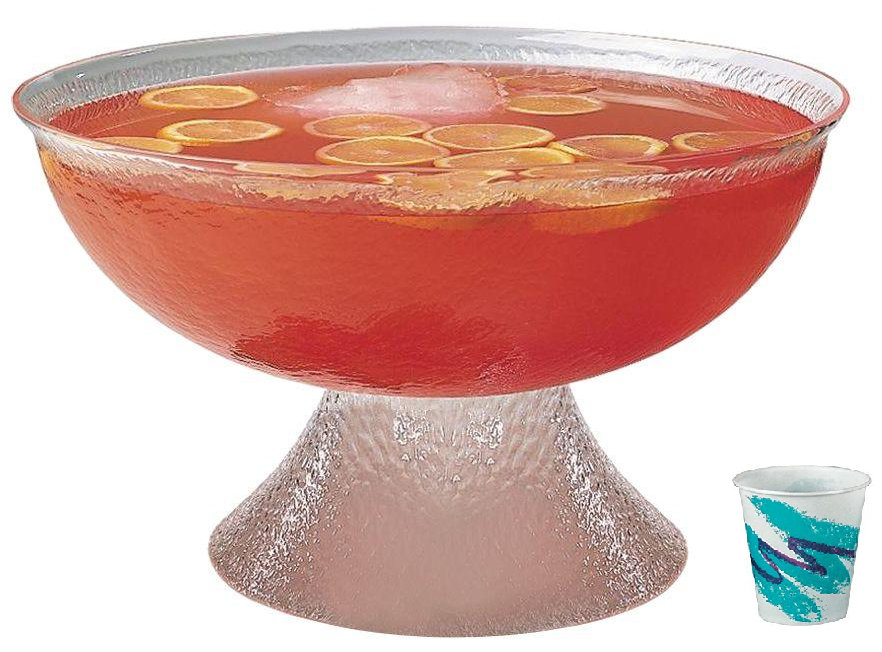
\includegraphics[scale=0.4]{Punch}
\caption{A punch bowl and a small Dixie cup.}
\label{Punch}
\end{figure}

In practice, worries of catastrophic slow-down from repeated buffer repacking are \emph{entirely warranted}. The rendering slow down is extensive and essentially defeats any 
gains we might make by rendering the data incrementally. Buffer repack is a barrier that may not be easily surmountable. I have found that we repeatedly are hampered by this issue. 
An initial implementation of the shelling method encountered rendering slow downs that led to around a 20-fold reduction in the 
frames-per-second values for any given volume. Such loss of render speed is more than just non-trivial; it is cataclysmic.  


\subsubsection{Current choice of $\sigma_k$ too weak} I also worry that using $\alpha_{\min}$ to calculate $\sigma_k$ will not create enough of a decrease in the inner shell Z-
levels. This is why it would be better to have a 
collection of scalars that take into account location of the brick relative to the texture. The challenge will be doing this \emph{without} being able to ``see" the volume prior to 
actually rendering the current shell. Another worry along these same lines deals with having to know all of the $\alpha$-values from a given render stage. In order to know 
percentiles, means, locations, etc., we must have a way of storing the entire matrix $\mathcal{A}$ and then, moreover, \emph{perform calculations on that matrix in the shader.} The 
capabilities of the shader are somewhat limited when it comes to performing calculations on matrices and determining global outcomes. Due to the multi-threaded aspect of much of 
the shader workflow, global calculations are costly and often times functionally prohibitive.    

\subsubsection{Incorrect blending of bricks in different shells}\label{badBlend} 
One more challenge that I see will be the issue of blending the layers of the render together. In the original implementation of the compute shader, brick data was fully loaded 
into buffer space. This allowed for each ray to independently access brick data \emph{as it encountered it}. Each pixel of the rendering could be blended smoothly as we moved from 
the origin of the ray outward. However, when a volume is rendered by means of shells, blending may not be as easy.  I will now refer several times to Figure \ref{Shell_Issue}. 
Figure \ref{Shell_Issue} demonstrates a basic ray-trace through a volume consisting of nine bricks. Only five of the bricks ($B_0$, $B_1$, $B_2$, $B_3$, and $B_4$, as labeled in 
the figure) are visible when the volume is viewed directly from above. The  remaining four bricks are entirely occluded by bricks $B_1$ through $B_4$ and are not depicted. We will 
not consider these occluded bricks further. 



In Figure \ref{Shell_Issue}, brick $B_0$ is intersected by three rays. Ray 1 intersects $B_0$ before intersecting with any other bricks (Ray 1 in fact intersects with no other 
bricks). This means that $B_0$ is an element of $\mathcal{S}_0$. Ray 2 also intersects with $B_0$, but not before first passing through $B_2$. Because $B_0$ and $B_2$ will both be 
rendered in the same shell, Ray 2 will be able to correctly blend and render all intersecting voxels from $B_0$ and $B_2$ when $\mathcal{S}_0$ is rendered. However, Ray 3 passes 
through $B_2$ and $B_1$ (in that order) before passing through $B_0$.
When the pixel associated with Ray 3 is rendered, it will be given initial values from the rendering of $\mathcal{S}_0$. 
However, the rendering of $B_1$ as part of $\mathcal{S}_1$ will require blending the voxels of $B_1$ which intersect with Ray 3 with the previous RGB$\alpha$ value determined when 
rendering $\mathcal{S}_0$. 
As $B_1$ lies in front of $B_0$ with respect to Ray 3, it seems likely that the voxels of $B_0$ which lie on Ray 3 will be depicted with higher emphasis than they should be given. 
Figure \ref{Shell_Issue2} shows one possible visual interpretation of what is happening. When $B_1$ is rendered as part of $\mathcal{S}_1$, bricks $B_0$ and $B_2$ have already been 
rendered. Because the RGB$\alpha$ values associated with the voxels of $B_0$ that are intersected by Ray 3 are originally rendered as if there is an empty space where $B_1$ will 
sit, the intensity of these values overall  may be overstated. Conversely, the RGB$\alpha$ values of $B_1$ may be understated in this instance. 

\begin{figure}[H]
\centering
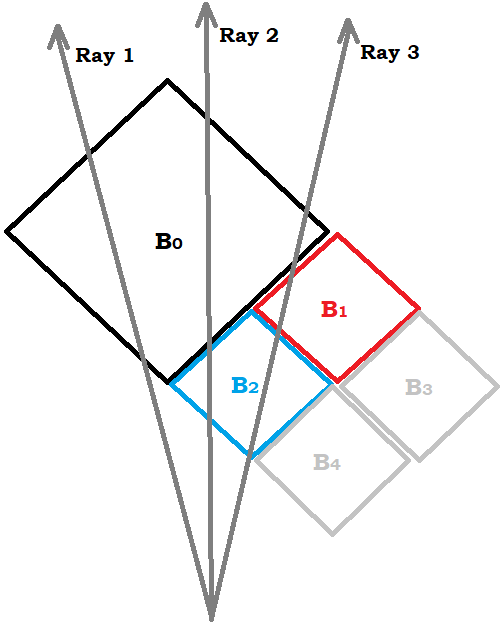
\includegraphics[scale=0.755]{Shell_Issue}
\caption{An overhead view of ray-tracing through several bricks. This figure demonstrates the various orders that a given brick can be ``seen" by ray-tracing.}
\label{Shell_Issue}
\end{figure}

\begin{figure}[H]
\centering
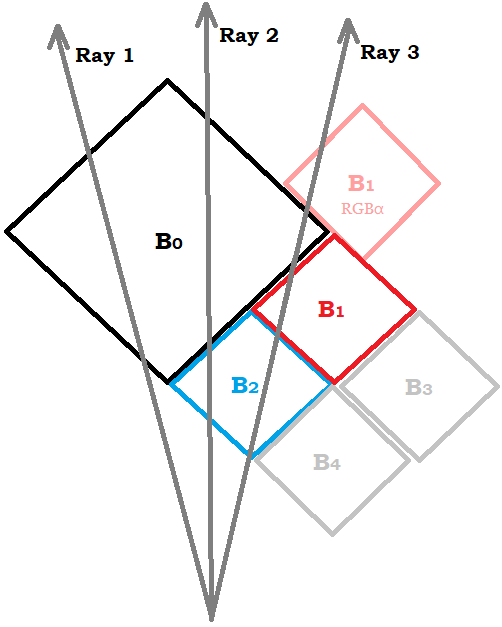
\includegraphics[scale=0.755]{Shell_Issue2}
\caption{An overhead view of ray-tracing through several bricks. This figure demonstrates a possible depiction error. Brick $B_1$ is shown in its actual position in the volume 
(solid red), as well as in a position (pink, with RGB$\alpha$ annotation) emulating an erroneous blending of the RGB$\alpha$ values associated with the voxels intersected by Ray 3. 
Compare with Figure \ref{Shell_Issue}}
\label{Shell_Issue2}
\end{figure}

This simple example could be extended arbitrarily to as many shells as desired by subdividing the smaller bricks ($B_1$ through $B_4$) into even smaller bricks. With enough 
subdivisions of the bricks into smaller bricks, we can create a situation where $B_0$  is in $\mathcal{S}_0$, yet has voxels which lie on some ray that has already passed through 
$k$-many bricks contained in $(k-1)$-many distinct shells.  


\section{Streaming volume data via SIEVAS}\label{SIEVAS} A more ideal work flow for rendering large-scale volumes will avoid the direct use of static data buffers all together. One way of doing 
this is a framework in which brick data is streamed directly from file. This would allow us to only read in brick data that is actually needed, and moreover, read in such data only 
at the Z-level requisite for its location relative to the eye of the viewer. Sadly, however, these overall ideas are likely not attainable with SIEVAS as it stands currently (January 8, 2019). I do not know of a solution that allows us to entirely forego the use of static buffers. See the discussion at subsection \ref{steamOne} for current thoughts on the matter.  

\subsection{Using the control and data topics}
SIEVAS is a data streaming platform built on a publisher-subscriber (PS) framework using a variety of brokers and messaging libraries 
(depending on the version of SIEVAS used, ActiveMQ, ZeroMQ, and JeroMQ are all used).  See \cite{LIVE} and \cite{SIEVAS} for further details on using SIEVAS. (LIVE in \cite{LIVE} is an early predecessor to SIEVAS).  The PS framework uses two topics: a \emph{control} topic and a \emph{data} topic. 
The control topic is used for any messaging that is not directly transferring brick data. The data topic is used exclusively for the transfer of actual data.  


\subsection{LOD culling with SIEVAS}
As a preliminary plan, we hope to be able to use an aggregated-$\alpha$-based culling method like unto that described at \ref{voxelLevel}. 
When the associated ray-trace is performed, each data point required for the ray-trace can be sampled by streaming the correct LOD for the given voxels. The data streaming platform 
that we will use is the Scientific \& Intelligence Exascale Visualization Analysis System (SIEVAS) created by Idaho National Labs. As has been mentioned before, it is imperative 
that SIEVAS allows for accessing voxel data at arbitrary Z-levels \emph{without} a priori \emph{knowing the ``correct" LOD for the given brick.} Global pre-passes to determine a 
uniform LOD for an entire brick can be costly and counter productive.  (Jan. 8, 2019) As I have learned more about SIEVAS, I have found that SIEVAS (which uses \texttt{BufferedFileReader} objects in Java to read the data files) does not allow for random-access-like attainment of single byte data. The entire idea of using SIEVAS to solve issues of buffer packing is ultimately not realizable I feel.   



\subsubsection{Current thoughts on using SIEVAS (Jan. 8, 2019)}


I am currently of the opinion that any compute shader method that relies on first knowing the ``correct" LOD for a brick before loading that brick into buffer space will likely 
end up being a pipe dream. One cannot both know the desired render level of a brick while at the same time avoid loading the brick into buffer space.  This will also mean that we 
cannot stream individual bricks (via SIEVAS or otherwise) and render them independent of one another. The bricks act as an associated system and cannot be viewed as entirely 
independent entities. The major question that must be addressed is as follows: How can one \emph{know} what LOD a brick needs to be streamed at without seeing that brick's role in 
the entirety of the volume? By my observation, there yet remains a large amount of misconception on this topic. There is no way that I am aware of that we can dynamically know the 
Z-level that a given brick \emph{should} be rendered at without rendering each brick at arbitrarily high levels. 




As of right now, it seems that perhaps one of the only meaningful reasons for even attempting to implement LOD culling when using SIEVAS would be to reduce
the amount of bytes that SIEVAS must 
read in order to obtain the voxel values we need. However, being as it is know before requesting the voxel data where in buffer the voxel data is located (this is calculated by a 
fixed algorithm), it may be just as easy to render every requested voxel at maximal Z-level. If it was just as easy (in terms of computational expenditures and memory use)
to access a voxel in a 
brick at Z-level one as it is to access a voxel in a brick at Z-level nine, there may be no reason to render a voxel at Z-level one anyway. (I.e. why render at level $z= 1$ when you can just as easily render at $z = 9$?)   
Location of the data point in the streaming buffer is not a matter of doing a linear search. Accessing a specific data point should be $\mathcal{O}(1)$. In practice, since we must read into the file linearly each and every time we want to access a single byte, any method which requires streaming data as single bytes will be prohibitively slow.    


One other potential reason for still observing LOD culling could be the possibility of the aggregated $\alpha$-value for a ray reaching saturation ($\alpha = 1$) more quickly. This 
thought is based on the hypothesis that rendering bricks (or portions of bricks) at lower Z-levels will lead to fewer voxels being rendered as transparent (or even just with lower 
$\alpha$-values). Lower Z-levels tend to emphasize opaque aspects of the brick and omit or de-emphasize the transparent portions. While there are instances where rendering a brick 
at a lower Z-level leads to specific voxels in that brick being given a lower $\alpha$-value, the overall outcome of rendering voxels at a lower Z-level seems to holistically 
lead to increases in the $\alpha$-values associated with those voxels. (This is anecdotal, not axiomatic). 
If a ray reaches $\alpha$-value saturation more quickly, this can lead to a more rapid termination of the ray-tracing process overall.
Empirical observations of the effects of LOD culling when streaming the brick data lead me to believe that  \emph{no substantive speedup is obtained by LOD culling}. However, in the case of the Gray Rot data, the ability to enforce some form of $\alpha$-based culling is rather useful when trying to isolate the true volume data from padding and extraneous voxels. 

\section{Summary of foreseen issues with compute shader rendering}\label{issues}
 This section provides an overview of the challenges and issues I see in using a compute shader. This is to provide an overall understanding of the issues of rendering a large scale volume using a compute shader.  Some of the thoughts presented here are repeating what has been said in previous sections. This is done in an attempt to gather all thoughts on volume visualization into a summary section. 
 
 \subsection{Lack of buffer space}
 As has been mentioned previously, because the compute shader relies on reading data via buffers, it may prove impossible to load large data sets into buffer space and render them.
This is the case with the IQ stations and the Gray Rot data (24 GB). Of the 324 total bricks in the volume, 180 of the bricks in the Gray Rot volume are of dimension $512 \times 512 \times 512$, which yields a maximal Z-level of nine. The remaining 144 bricks are of dimension $256 \times 256 \times 256$, which yields a maximal Z-level of eight. If \emph{all} bricks in Gray Rot are rendered at $z = 8$, then we only have roughly 3 GB of volume data, which is in fact renderable on a desktop machine.  Thus if we render every brick at level $z=8$ or lower for Gray Rot, buffer overflow does not become an issue. (I have successfully  done so on several occasions. Note that it takes about a minute to actually read in and load the data once you press play in Unity). It should of course be noted that there is no magical formula for rendering massive amounts of data in minuscule amounts of time. We are not capable of taking 30, 40,..., 100 GB  (or whatever size we dream of) of high density data and producing in a matter of seconds a rendering that is high resolution  as well as dynamically alterable.  

\subsection{Determination \emph{a priori} of requisite LOD}
The main aim of rendering certain bricks at lower LOD is to pare down the amount of data that must be loaded into buffer space. 
From a theoretical perspective, there is great salience 
in loading partially or fully occluded bricks at low Z-levels. 
Such a practice allows for faster rendering of a volume by reducing how much work must go into displaying voxels which are not visible to the user. 
However, the question then must be asked: how does one determine \emph{a priori} the requisite LOD for each brick individually? 
Unlike static images, which can be rendered in predetermined layers, we are attempting to render a volume whose orientation can be dynamically changed. A static image can have predetermined layers based on a fixed vantage point; a dynamically changing volume does not avail such predetermination. 


Furthermore, there is no inherent pattern to the order which the bricks of a volume are seen in. This means that any LOD culling algorithm that is contingent on knowing how far from the camera a given brick is \emph{before loading that brick into buffer} will be dependent on an algorithmic approach that will essentially amount to chasing our tail in a never ending circle.   Thus, without first performing some sort of pre-pass of the volume in its
current orientation in order to establish a hierarchy of visibility for the bricks (a process which is computationally expensive), there is no way of knowing what level
each brick must be initially rendered at. We can refer to this as ``lack of oracle knowledge" 
(meaning, there is no crystal ball that can tell us what Z-level is necessary for properly rendering each brick). Prescient volume rendering is, to be blunt, unfeasible and based on the acquisition of an ultimately chimerical LOD culling algorithm. 

One proposed approach to LOD culling that I will discuss briefly is that of render all bricks at level $z = 0$ (or $z= 1, 2,$ etc.; a predetermined ``low" Z-level) and ramp up the Z-levels as necessary.  This then again causes us to beg the question as to determining an algorithm for settling on the ``correct" LOD for a given brick. Lack of oracle knowledge rears it's head again!  Moreover,  rendering a brick at too low of a Z-level will introduce false occlusions that would not be present in a properly rendered volume. 

In \cite{PEARC18}, the authors suggest that we ``adjust the level of detail of each data brick depending on the location of the brick relative to the camera." This is even more na\"{i}ve of an approach to LOD culling than $\alpha$-based culling. 
There are of course many volumes for which some bricks that are close to the camera are mere padding for the volume.  Should these padding bricks (even if uniformly transparent ($\alpha = 0$)) affect the LOD for ``true" data bricks which lie behind the padding bricks? It is an extremely easy exercise to construct examples where culling solely on brick location relative to the camera will lead to too low a LOD for bricks occluded by padding and bricks with little substantive volumetric information. Culling LOD based on camera location also does nothing to overcome the issues of having to globally prepass the volume to determine brick LOD before loading brick data into buffer. The related issue of repeated buffer repack is similarly not solved in the slightest. 


\subsection{Streaming data bricks one at a time}\label{steamOne} As has been addressed before, a volume does not consist of independent bricks, but rather a system of co-dependent bricks. The 
current plan to render bricks one at a time will likely be \emph{very difficult} to make work properly. Brick voxel blending will likely be incorrect 
(see \ref{badBlend} for example) 
when we do not render the bricks as a system. While it may be \emph{theoretically} feasible to ameliorate some of the issues of blending by rendering bricks in an
 order like unto that suggested by the shelling method above, note that the overall problem is not solved. (As the discussion at \ref{badBlend} indicates). That is to say,
 while it is better to render the bricks in an orientation-guided order (as opposed to a naive $0,~1,~2,\ldots$ ordering), incorrect blending will still occur. This will be 
 exacerbated by the fact that, unlike in the original shells method, we will not be rendering bricks in layers, but one at a time. This will introduce even further issues with the 
 layering of bricks that lie in the same shell, but for which one brick partially covers another. 
 
 The very best set up in terms of byte data access would be to use a SQL data base to hold the data and have the SIEVAS message system request specific points using SQL queries. 
 The data could then be passed one int at a time. We will likely need to hold the data in SQL databases that are on a brick basis (i.e. something like 
 \verb|volume_v_brick_b.sql| 
 where \texttt{v} and \texttt{b} would be the volume and brick numbers respectively). However, holding all the data in one big database causes \emph{extensive} data bloat, since much of the 
 column data is exactly the same (i.e. just a repeating of the volume name and brick number millions of times). I have attempted to use a SQL database to store the Visible Male dataset; it was an abject failure. There would be no way that we could possibly work with the amount of storage on disk that would be required to place these volumes in an indexed SQL database. 
 
 \emph{The reality is that we would be very best served by being able to have all the data in buffer. There is no way around that. } 
 It just feels like we are trying to magically bake chocolate chip cookies one ingredient at a time. It just doesn't really work. 
 Sure, you can pour the sugar into the bowl separately from the flour and the eggs. But you have to mix them at some point. 
 We cannot process and render a single brick and then render another brick entirely independently of the first brick. 
 You cannot just pour eggs, flour, sugar, and chocolate chips onto four separate pans and bake them to get chocolate chip cookies. It does not work like that.  
 
 In summary, I have found no feasible way to render a dynamic volume one brick at a time. Issues of blending cannot be fixed without substantive loss of rendering speed (if the blending issues could even be fixed at all). Moreover, there is no way to determine a ``correct" LOD for a given brick without first rendering the entire volume at the highest available LOD (which would defeat the purpose of rendering a volume one brick at a time, with each brick being rendered at a predetermined ``correct" LOD). 
 
\subsection{Repeated repacking of data into buffers} There is no way around the fact that a compute shader requires the use of buffers. (This has been well established). As currently implemented, the volume visualizer tool packs the buffers once (at initialization) and once only. However, in order to fully utilize the benefits of LOD culling, every time that the orientation of the volume changes, the buffers must be repacked to account for changes in ``correct" Z-level of each brick. Note that due to the difficulty of actually determining when the volume has been moved, we must re-render the volume repeatedly, even when the user has not changed the orientation of the volume. Hence, the render sequence would need to check for changes in Z-level at every frame and then repack the buffer each and every time when necessary. Preliminary attempts at doing this were not at all promising.  The bulk of this issue in regards to LOD determination is addressed in \ref{repack} and I will direct readers there for further thoughts on the matter. 

Buffer repack is also a significant issue when we stream the volume data. Essentially the same challenges as before will still present themselves. (All we have really changed is the source that the data is coming from. Once it is loaded in buffers, the complications of buffer repack are much the same as before). 

One idea that was presented was to only repack the buffer if a brick needs to be rendered in higher detail than before, but to retain any brick data in the buffer if the associated brick is being rendered at a level at or lower than the available detail in the buffer. This approach, however, will be extremely hard to keep track of (let's face it, it's sloppy and chaotic) and will lead to the overlying issue of buffer overflow once again. At some point, the buffer would become overly saturated with brick data at too high of a Z-level. (Just move the volume around in a circle a few times and we will have rendered many of the bricks at high levels). 

\subsection{Limits on the number of initialized buffers}
In DirectX-HLSL (language used to write compute shaders), a shader can only have eight of what are called ``unordered access views" (UAVs). From the \href{https://docs.microsoft.com/en-us/windows/desktop/direct3d12/typed-unordered-access-view-loads}{Microsoft website} we have: 
\begin{displayquote}
``An unordered access view (UAV) is a view of an unordered access resource (which can include buffers, textures, and texture arrays, though without multi-sampling). A UAV allows temporally unordered read/write access from multiple threads. This means that this resource type can be read/written simultaneously by multiple threads without generating memory conflicts."
\end{displayquote}
Specific to our use here, our shader requires a minimum of four UAVs:
\begin{itemize}
\item A \texttt{RWTexture2D<float4>} called \texttt{Result} which stores the accumulating and resulting texture matrix during the ray tracing process. 
\item A \texttt{RWStructuredBuffer<MetaBrick>} called  \texttt{\_MetaBrickBuffer} which holds the \texttt{MetaBrick} objects carrying the basic details of each brick (but not the actual raw brick data of course). 
\item A \texttt{RWStructuredBuffer<MetaVolume>} called  \texttt{\_MetaVolumeBuffer} which holds the \texttt{MetaVolume} object associated with the volume being rendered. Remember that we must pass almost \emph{everything} into the shader via buffers. Hence the reason we must devote an entire buffer just to holding a 64 byte  \texttt{MetaVolume} object.
\item At least one \texttt{RWStructuredBuffer<uint>} object which holds the actual raw data (packed as \texttt{uint}s). The number of data buffers that we have dictates how much actual data we can hold and render. 
\end{itemize}

Thus, in total, we can have a maximum of five \texttt{RWStructuredBuffer<uint>} objects for holding raw data. Although there does not seem to be any definitive source (i.e. from Microsoft or Unity themselves), it seems that the maximum buffer size is 2147483647 bytes ($2^{31} - 1$ bytes, which is 2 GB less a single byte). There are ways around this in C\# I believe; I am not aware of any way around this limit in HLSL. (This is not to say a way does not exist). Note that any buffer used in the shader was at one point a buffer in the volume controller. Thus, if we intend to set the \texttt{RWStructuredBuffer}s in the volume controller, buffer size limits are relevant for both C\# and HLSL. Overall, it seems that just less than 10 GB can be rendered when using a compute shader. I have not pushed this limit. If the software (soft limit) can be sidestepped, it is likely that the hardware exists to handle much more than 10 GB of volume buffer data. 


\section{Current State}\label{conclude}
As of January 25th, 2019, the current state of the volume visualizer is as follows:
\begin{itemize}
\item The current version of the volume visualizer is found in the \verb'VolViz_Stream' branch of the PRISM project. The README.md file therein describes the basic controls for the visualizer.
\item Only the desktop version of the visualizer currently works. Unity no longer supports older versions of libraries used to make the VR/CAVE versions of the visualizer. 
\item SIEVAS is implemented in this version of the visualizer. You will need to have SIEVAS installed and running if you wish to use the visualizer.
\item The visualizer currently uses $\alpha$-based culling as outlined in Subsection \ref{voxelLevel}. This allows for culling away some less useful pieces of the GreyRot data set. It does not reduce the amount of data that must be initially packed into buffer space. 
\item No aspect of shelling (see Section \ref{shells}) is being used. The volumes are rendered in their entirety, without the use of shells. 
\item The license and README information for PRISM have been sent to Wendy Skinner in Technology Deployment on January 17, 2019. She should be spearheading the public release of the software onto GitHub. 
\item Contact information: Randall Reese, randall.reese@inl.gov. 
\end{itemize}




%%% ************************************************************************************************************************************************************ 

%%%      Some comments and notes for future discussion.

%%% ************************************************************************************************************************************************************

%\section{Tasks To Do}
%\textsl{  
%\begin{itemize}
%\item Determine the shell that each brick falls into. Previously I was referring to this process as the ``render tree." \vspace*{0.5cm}
%\item Any brick seen by a ray as a 'first brick' is rendered first. Any brick seen by any ray as a 'second brick' (but not a 'first brick') is rendered subject to the alpha-value-
%based culling. In other words, render $\mathcal{S}_0$, $\mathcal{S}_1$, $\mathcal{S}_2, \ldots,$ $\mathcal{S}_{19}$ as discussed above. \vspace*{0.5cm}
%\item Do an overall algorithm where we render one shell at a time recursively (or iteratively), and do not reset the \texttt{Result} 
%matrix. Use it to set the \texttt{fColor} values for the next iteration.\vspace*{0.5cm}
%\item Note that we will need to back scale the \texttt{Result} values to remove the \texttt{\_normPerRay} scalar 
%value.\vspace*{0.5cm}
%\item Implement SIEVAS streaming. How does SIEVAS even work?
%\end{itemize}
%   }


% Appendix
%\appendix
%\section*{APPENDIX}
%\setcounter{section}{1}
% Bibliography
\bibliographystyle{ACM-Reference-Format-Journals}
\bibliography{LODrefs}
                                % Sample .bib file with references that match those in
                                % the 'Specifications Document (V1.5)' as well containing
                                % 'legacy' bibs and bibs with 'alternate codings'.
                                % Gerry Murray - March 2012

% History dates
\received{September 2018}{September 2018}{September 2018}


%%\elecappendix



\end{document}
% End of v2-acmlarge-sample.tex (March 2012) - Gerry Murray, ACM
